\documentclass[tikz, border=16pt]{standalone}
\usepackage{amsmath, amssymb}
\usetikzlibrary{arrows.meta, positioning}

\begin{document}
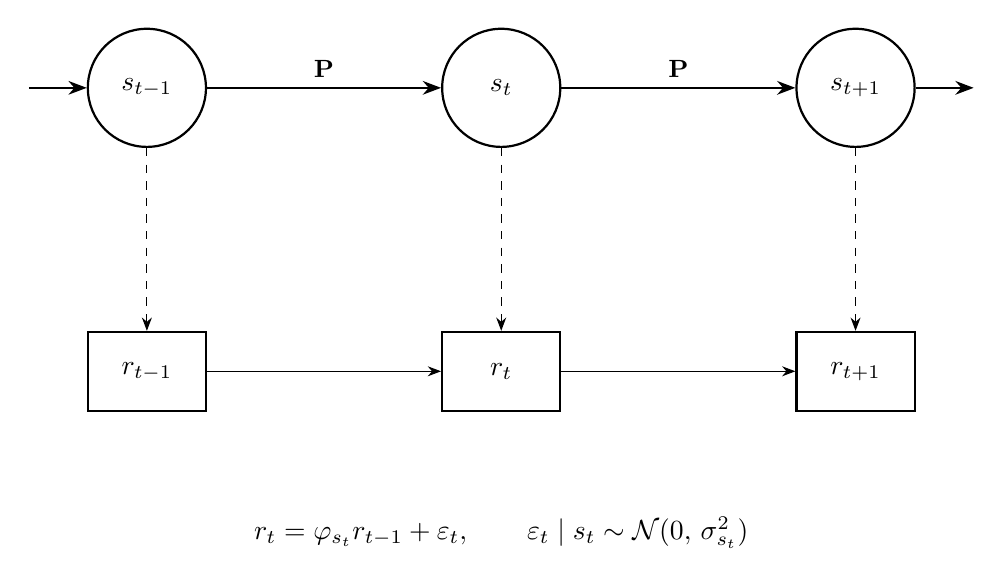
\begin{tikzpicture}[
  >=Stealth,
  thick,
  state/.style={
    circle, draw, fill=white,
    minimum size=1.5cm,
    font=\normalsize
  },
  obs/.style={
    rectangle, draw, fill=white,
    minimum width=1.5cm, minimum height=1.0cm,
    font=\normalsize
  },
]

  % -------------------------------------------------------
  %  Nodes
  % -------------------------------------------------------
  \node[state] (s1) at (0.0,  0) {$s_{t-1}$};
  \node[state] (s2) at (4.5,  0) {$s_t$};
  \node[state] (s3) at (9.0,  0) {$s_{t+1}$};

  \node[obs]   (r1) at (0.0, -3.6) {$r_{t-1}$};
  \node[obs]   (r2) at (4.5, -3.6) {$r_t$};
  \node[obs]   (r3) at (9.0, -3.6) {$r_{t+1}$};

  % -------------------------------------------------------
  %  Forward transitions (time flows left to right)
  % -------------------------------------------------------
  \draw[->] (-1.5, 0) -- (s1);
  \draw[->] (s1) -- node[above, font=\small]{$\mathbf{P}$} (s2);
  \draw[->] (s2) -- node[above, font=\small]{$\mathbf{P}$} (s3);
  \draw[->] (s3) -- (10.5, 0);

  % -------------------------------------------------------
  %  Emissions  (dashed)
  % -------------------------------------------------------
  \draw[->, dashed, thin] (s1) -- (r1);
  \draw[->, dashed, thin] (s2) -- (r2);
  \draw[->, dashed, thin] (s3) -- (r3);

  % -------------------------------------------------------
  %  AR(1) dependency between observations
  % -------------------------------------------------------
  \draw[->, thin] (r1) -- (r2);
  \draw[->, thin] (r2) -- (r3);

  % -------------------------------------------------------
  %  Emission model below figure
  % -------------------------------------------------------
  \node[below=1.2cm of r2, font=\normalsize] {
    $r_t = \varphi_{s_t} r_{t-1} + \varepsilon_t, \qquad
     \varepsilon_t \mid s_t \sim \mathcal{N}(0,\, \sigma_{s_t}^2)$
  };

\end{tikzpicture}
\end{document}
